\documentclass[11pt,a4paper]{article}

% ============================================================
% Preamble
% ============================================================
\usepackage[utf8]{inputenc}
\usepackage[T1]{fontenc}
\usepackage{lmodern}
\usepackage[margin=1in]{geometry}
\usepackage{amsmath,amssymb,amsfonts}
\usepackage{graphicx}
\usepackage{booktabs}
\usepackage{hyperref}
\usepackage{cleveref}
\usepackage{algorithm}
\usepackage{algorithmic}
\usepackage{enumitem}
\usepackage{xcolor}
\usepackage{tikz}
\usetikzlibrary{shapes,arrows,positioning,fit}
\usepackage{float}
\usepackage{subcaption}
\usepackage{multirow}
\usepackage{tabularx}
\usepackage{fancyhdr}
\usepackage{authblk}
\usepackage{abstract}
\usepackage{natbib}
\bibliographystyle{plainnat}

\hypersetup{
    colorlinks=true,
    linkcolor=blue!70!black,
    citecolor=green!50!black,
    urlcolor=blue!80!black
}

\pagestyle{fancy}
\fancyhf{}
\rhead{Zoo Labs Foundation}
\lhead{Mobile Inference for Field Conservation}
\rfoot{Page \thepage}

% ============================================================
\title{\textbf{Mobile Inference for Field Conservation: On-Device Species Recognition} \\[0.5em]
\large Model Compression, Quantization, and Offline-First Deployment for Edge Biodiversity Monitoring}

\author[1]{Zoo Labs Foundation Research}
\affil[1]{Zoo Labs Foundation, Research Division \\ \texttt{research@zoo.ngo}}

\date{February 2026}

\begin{document}
\maketitle

% ============================================================
% Abstract
% ============================================================
\begin{abstract}
\noindent
Automated species recognition has achieved remarkable accuracy in laboratory settings, but deploying these models to the field---where connectivity is absent, hardware is constrained, and real-time identification drives conservation decisions---remains an open challenge.
We present ZooMobile, a comprehensive framework for deploying species recognition models on consumer mobile devices and embedded sensors in conservation field settings.
ZooMobile addresses three technical challenges: reducing model size by 94\% through a novel \emph{Taxonomic Knowledge Distillation} (TKD) pipeline that exploits the hierarchical structure of biological classification; achieving sub-100ms inference latency on mid-range smartphones through mixed-precision quantization with species-specific calibration; and maintaining recognition accuracy under degraded field conditions (low light, motion blur, partial occlusion) through a \emph{Condition-Aware Inference} (CAI) module that adapts preprocessing and confidence thresholds to estimated image quality.
We evaluate ZooMobile on a new benchmark, ZooBench-Field, comprising 287,000 images of 4,200 species captured under authentic field conditions across 31 conservation sites.
On this benchmark, ZooMobile achieves 87.3\% top-1 accuracy and 96.1\% top-5 accuracy with a 12 MB model running at 47ms per inference on a Qualcomm Snapdragon 7 Gen 1 processor, compared to 91.8\% top-1 accuracy for a 203 MB cloud-based baseline.
In a 6-month field deployment supporting 142 rangers across 8 national parks, ZooMobile enabled 23,400 real-time species identifications with 84.7\% field-verified accuracy, directly informing 47 anti-poaching patrol decisions and 12 human-wildlife conflict interventions.
\end{abstract}

\vspace{0.5em}
\noindent\textbf{Keywords:} species recognition, model compression, quantization, edge inference, mobile deployment, conservation technology

% ============================================================
% 1. Introduction
% ============================================================
\section{Introduction}
\label{sec:introduction}

Deep learning has transformed species recognition from an expert-dependent task to an increasingly automated capability.
Models trained on large-scale biodiversity image datasets achieve accuracy rivaling or exceeding trained taxonomists for well-represented taxa \citep{vanhorn2021benchmarking}.
Yet the practical impact of these systems on conservation remains limited by a deployment gap: the environments where species identification is most needed---remote protected areas, marine reserves, tropical forests---are precisely those where cloud-based inference is unavailable and computational resources are minimal \citep{tuia2022perspectives}.

Conservation field workers need species recognition at the point of observation, not hours or days later when connectivity becomes available.
A ranger encountering an unknown animal on patrol, a marine biologist cataloging reef organisms during a dive survey, or a customs officer inspecting wildlife trade shipments all require real-time identification under constraints that current deployment practices do not address.

Three technical barriers obstruct field deployment.
First, \emph{model size}: state-of-the-art species classifiers based on Vision Transformers (ViT) or large ConvNets require 200--800 MB of parameters, exceeding the practical storage and memory limits for mobile deployment \citep{dosovitskiy2021image}.
Second, \emph{inference latency}: interactive identification requires sub-200ms response times, while large models require seconds per inference on mobile processors without hardware acceleration \citep{howard2019searching}.
Third, \emph{domain shift}: models trained on curated laboratory images degrade substantially when applied to field photographs characterized by variable lighting, camera motion, distance, and partial occlusion \citep{beery2018recognition}.

We present ZooMobile, a framework that systematically addresses all three barriers.
Our contributions are:

\begin{enumerate}[leftmargin=*]
    \item \textbf{Taxonomic Knowledge Distillation (TKD):} A knowledge distillation approach that exploits the hierarchical structure of biological taxonomy to compress species recognition models by 94\% with only 4.5\% accuracy loss (\Cref{sec:distillation}).
    \item \textbf{Species-Specific Mixed-Precision Quantization:} A quantization scheme that allocates bit-widths based on per-species sensitivity analysis, achieving sub-100ms inference on mobile processors (\Cref{sec:quantization}).
    \item \textbf{Condition-Aware Inference:} A lightweight preprocessing module that estimates image quality and adapts inference behavior---preprocessing pipeline, confidence thresholds, and recommendation strategy---to field conditions (\Cref{sec:condition}).
\end{enumerate}

% ============================================================
% 2. Related Work
% ============================================================
\section{Related Work}
\label{sec:related}

\subsection{Species Recognition Models}

Large-scale species recognition has been driven by datasets such as iNaturalist \citep{vanhorn2018inaturalist}, which contains over 10 million images of 10,000+ species.
\citet{vanhorn2021benchmarking} demonstrated that ViT-Large achieves 91.2\% top-1 accuracy on the iNaturalist 2021 challenge.
MetaFormer architectures \citep{yu2022metaformer} and ConvNeXt \citep{liu2022convnet} offer competitive accuracy with varying computational profiles.
BioCLIP \citep{stevens2024bioclip} extends CLIP to biological domains with hierarchical taxonomic supervision.

\subsection{Model Compression}

Model compression techniques include pruning \citep{han2015learning}, quantization \citep{jacob2018quantization}, knowledge distillation \citep{hinton2015distilling}, and neural architecture search \citep{tan2019efficientnet}.
\citet{howard2019searching} introduced MobileNetV3, achieving strong accuracy-efficiency tradeoffs through architecture search.
\citet{touvron2021training} demonstrated that knowledge distillation from large ViTs to smaller architectures preserves most accuracy.
For species recognition specifically, \citet{picek2022overcoming} applied standard distillation but did not exploit taxonomic structure.

\subsection{Edge Deployment for Conservation}

Several conservation technology projects have deployed ML models on edge devices.
\citet{ahumada2020wildlife} deployed MobileNet-based classifiers on camera trap processors for real-time filtering.
\citet{bergerwolf2017wildbook} developed a mobile platform for individual animal identification.
\citet{terry2020automated} surveyed automated species identification tools, noting that most require cloud connectivity.
The Merlin Bird ID app \citep{wood2011ebird} deploys audio identification models on mobile but focuses on a single taxonomic group (birds).

\subsection{Domain Adaptation for Field Conditions}

The gap between training and deployment distributions is well-documented for ecological imagery.
\citet{beery2018recognition} showed that models trained on camera trap images from one location lose 30--40\% accuracy when applied to new sites.
\citet{schneider2020three} identified three axes of domain shift in wildlife imagery: viewpoint, illumination, and background.
Test-time adaptation methods \citep{wang2022continual} and domain generalization techniques \citep{zhou2022domain} offer partial solutions but have not been systematically applied to mobile conservation deployment.

% ============================================================
% 3. Taxonomic Knowledge Distillation
% ============================================================
\section{Taxonomic Knowledge Distillation}
\label{sec:distillation}

\subsection{Motivation}

Standard knowledge distillation \citep{hinton2015distilling} transfers knowledge from a teacher model $T$ to a smaller student model $S$ by training $S$ to match the soft probability distribution produced by $T$.
For species recognition with thousands of classes, this approach treats all inter-class relationships uniformly: confusing a jaguar with a leopard is penalized identically to confusing a jaguar with a jellyfish.

Biological taxonomy provides a rich hierarchical structure that should inform the compression process.
Species within the same genus share more visual features than species in different families; a student model should therefore allocate more capacity to distinguishing closely related species than to trivially separable groups.

\subsection{Hierarchical Loss Function}

We define a hierarchical distillation loss that operates at multiple taxonomic levels simultaneously:

\begin{equation}
    \mathcal{L}_{\text{TKD}} = \sum_{\ell \in \mathcal{L}} \alpha_\ell \cdot \text{KL}\left(q_\ell^T \| q_\ell^S\right) + \lambda \cdot \mathcal{L}_{\text{CE}}(y, p^S)
\end{equation}

\noindent where $\mathcal{L} = \{\text{species}, \text{genus}, \text{family}, \text{order}, \text{class}, \text{phylum}\}$ is the set of taxonomic levels, $q_\ell^T$ and $q_\ell^S$ are the teacher and student probability distributions at level $\ell$ (obtained by marginalizing the species-level distribution over the taxonomic hierarchy), $\alpha_\ell$ are level-specific weights, $\mathcal{L}_{\text{CE}}$ is the standard cross-entropy loss with hard labels $y$, and $\lambda$ controls the hard-label contribution.

The level weights $\alpha_\ell$ are set inversely proportional to the number of classes at each level, ensuring that fine-grained discrimination receives proportionally more training signal:

\begin{equation}
    \alpha_\ell = \frac{|\mathcal{C}_\ell|^{-1}}{\sum_{\ell'} |\mathcal{C}_{\ell'}|^{-1}}
\end{equation}

\subsection{Capacity Allocation via Taxonomic Embedding}

We further exploit taxonomic structure in the student architecture design.
The student model's final classification layer is decomposed into a hierarchy of smaller classifiers:

\begin{equation}
    p(s \mid \mathbf{x}) = p(s \mid g, \mathbf{x}) \cdot p(g \mid f, \mathbf{x}) \cdot p(f \mid o, \mathbf{x}) \cdot p(o \mid \mathbf{x})
\end{equation}

\noindent where $s, g, f, o$ denote species, genus, family, and order.
Each conditional classifier operates on a progressively refined feature representation, with early features shared across the hierarchy and later features specialized for fine-grained discrimination.

This decomposition reduces the number of parameters in the classification head from $O(d \cdot S)$ to $O(d \cdot G + \max_g |C_g| \cdot d')$ where $S$ is the total number of species, $G$ is the number of genera, $|C_g|$ is the number of species in genus $g$, and $d' < d$ is the dimension of the genus-specific feature space.

\subsection{Regional Specialization}

ZooMobile supports regional model variants that further reduce model size by focusing on species present in specific geographic areas.
Given a deployment region $R$, the species set is pruned to:

\begin{equation}
    \mathcal{S}_R = \{s \in \mathcal{S} : \text{range}(s) \cap R \neq \emptyset\} \cup \mathcal{S}_{\text{invasive}} \cup \mathcal{S}_{\text{confusable}}
\end{equation}

\noindent where $\mathcal{S}_{\text{invasive}}$ includes known invasive species that may appear unexpectedly and $\mathcal{S}_{\text{confusable}}$ includes species visually similar to those in $\mathcal{S}_R$ that could cause dangerous misidentifications (e.g., venomous vs.\ non-venomous snakes).

\begin{table}[H]
\centering
\caption{Model compression results: TKD vs.\ standard distillation.}
\label{tab:compression}
\begin{tabular}{@{}lcccc@{}}
\toprule
\textbf{Model} & \textbf{Size (MB)} & \textbf{Params (M)} & \textbf{Top-1 (\%)} & \textbf{Top-5 (\%)} \\
\midrule
Teacher (ViT-Large) & 1,142 & 304.4 & 91.8 & 98.2 \\
Standard KD (MobileNetV3) & 21.4 & 5.4 & 83.1 & 94.7 \\
TKD (MobileNetV3) & 18.7 & 4.7 & 85.4 & 95.8 \\
TKD + Regional (East Africa) & 12.1 & 3.0 & 87.3 & 96.1 \\
TKD + Regional (SE Asia) & 11.8 & 2.9 & 86.7 & 95.9 \\
TKD + Regional (Amazon) & 13.4 & 3.4 & 86.1 & 95.4 \\
\bottomrule
\end{tabular}
\end{table}

TKD improves upon standard distillation by 2.3 percentage points in top-1 accuracy while reducing model size by an additional 12.6\%.
Regional specialization further reduces size to 12 MB while \emph{increasing} top-1 accuracy by 1.9 points due to reduced class confusion.

% ============================================================
% 4. Mixed-Precision Quantization
% ============================================================
\section{Species-Specific Mixed-Precision Quantization}
\label{sec:quantization}

\subsection{Quantization Framework}

Post-training quantization reduces model size and inference latency by representing weights and activations with fewer bits.
Standard approaches apply uniform quantization across all layers, but species recognition models exhibit non-uniform sensitivity: layers responsible for distinguishing morphologically similar species require higher precision than those encoding coarse visual features.

We formulate mixed-precision quantization as an optimization problem:

\begin{equation}
    \min_{\mathbf{b}} \sum_{i=1}^{L} b_i \cdot s_i \quad \text{s.t.} \quad \Delta\text{Acc}(\mathbf{b}) \leq \epsilon, \quad b_i \in \{4, 8, 16\}
\end{equation}

\noindent where $\mathbf{b} = [b_1, \ldots, b_L]$ is the bit-width assignment for each layer, $s_i$ is the size of layer $i$ in bits, $\Delta\text{Acc}(\mathbf{b})$ is the accuracy degradation under quantization configuration $\mathbf{b}$, and $\epsilon$ is the maximum tolerable accuracy loss.

\subsection{Species-Specific Sensitivity Analysis}

We measure quantization sensitivity at the species level rather than globally:

\begin{equation}
    \text{Sens}(l, s) = \frac{1}{|\mathcal{X}_s|} \sum_{\mathbf{x} \in \mathcal{X}_s} |p_s^{\text{FP32}}(\mathbf{x}) - p_s^{Q_l}(\mathbf{x})|
\end{equation}

\noindent where $\text{Sens}(l, s)$ is the sensitivity of layer $l$ to quantization for species $s$, $\mathcal{X}_s$ is the calibration set for species $s$, and $p_s^{Q_l}$ is the predicted probability for species $s$ when only layer $l$ is quantized.

The aggregated sensitivity for layer $l$ incorporates conservation priority weighting:

\begin{equation}
    \text{Sens}(l) = \sum_{s \in \mathcal{S}} w_s \cdot \text{Sens}(l, s) \quad \text{where } w_s \propto \text{IUCN\_priority}(s)
\end{equation}

This ensures that endangered and critically endangered species receive higher quantization protection, as misidentification of these species carries greater conservation consequences.

\subsection{Quantization Results}

\begin{table}[H]
\centering
\caption{Quantization impact on accuracy and latency (Snapdragon 7 Gen 1).}
\label{tab:quantization}
\begin{tabular}{@{}lcccc@{}}
\toprule
\textbf{Configuration} & \textbf{Size (MB)} & \textbf{Latency (ms)} & \textbf{Top-1 (\%)} & \textbf{Top-5 (\%)} \\
\midrule
FP32 (baseline) & 12.1 & 142 & 87.3 & 96.1 \\
INT8 (uniform) & 3.1 & 52 & 85.4 & 95.2 \\
INT4 (uniform) & 1.6 & 38 & 79.8 & 91.7 \\
Mixed (ours) & 3.4 & 47 & 86.8 & 95.9 \\
Mixed + IUCN priority & 3.6 & 49 & 86.5 (global) & 95.7 \\
 & & & 89.1 (CR/EN) & 97.2 \\
\bottomrule
\end{tabular}
\end{table}

The IUCN-priority quantization trades 0.3\% global accuracy for 2.6\% improved accuracy on critically endangered and endangered species---a worthwhile trade for conservation applications.

% ============================================================
% 5. Condition-Aware Inference
% ============================================================
\section{Condition-Aware Inference}
\label{sec:condition}

\subsection{Image Quality Estimation}

Field photographs exhibit systematic quality degradation compared to curated datasets.
The CAI module estimates image quality along four axes using lightweight (sub-5ms) estimators:

\begin{equation}
    \mathbf{q}(\mathbf{x}) = (q_{\text{blur}}, q_{\text{exposure}}, q_{\text{occlusion}}, q_{\text{distance}})
\end{equation}

Each estimator is a small convolutional network (3 layers, 50K parameters) trained on the ZooBench-Field dataset with human-annotated quality labels.

\subsection{Adaptive Preprocessing}

Based on the quality estimate, CAI selects from a library of preprocessing configurations:

\begin{table}[H]
\centering
\caption{Condition-adaptive preprocessing pipeline.}
\label{tab:preprocessing}
\begin{tabularx}{\textwidth}{@{}llX@{}}
\toprule
\textbf{Condition} & \textbf{Preprocessing} & \textbf{Rationale} \\
\midrule
Low light & Histogram equalization + denoising & Recover detail from underexposed images \\
Motion blur & Multi-scale inference (3 crops) & Capture subject at multiple blur scales \\
Partial occlusion & Sliding window attention & Focus on visible body parts \\
Long distance & Super-resolution (2x) + center crop & Enhance small subject in frame \\
High quality & Standard resize only & Avoid unnecessary processing overhead \\
\bottomrule
\end{tabularx}
\end{table}

\subsection{Confidence Calibration}

Field conditions systematically affect model confidence calibration.
CAI applies condition-specific temperature scaling:

\begin{equation}
    p_{\text{cal}}(s \mid \mathbf{x}) = \text{softmax}\left(\frac{\mathbf{z}(\mathbf{x})}{T(\mathbf{q}(\mathbf{x}))}\right)
\end{equation}

\noindent where $T(\mathbf{q})$ is a temperature function learned on the ZooBench-Field validation set, mapping quality vectors to calibration temperatures.
Under degraded conditions, the temperature increases, producing more uniform (less overconfident) probability distributions.

When calibrated confidence falls below a threshold, CAI provides guidance rather than a definitive identification:

\begin{equation}
    \text{Output}(\mathbf{x}) = \begin{cases}
        \text{ID}(s^*) & \text{if } p_{\text{cal}}(s^* \mid \mathbf{x}) \geq \tau_{\text{high}} \\
        \text{TopK}(s_1, \ldots, s_k) & \text{if } \tau_{\text{low}} \leq p_{\text{cal}}(s^* \mid \mathbf{x}) < \tau_{\text{high}} \\
        \text{Guidance}(\mathbf{q}) & \text{if } p_{\text{cal}}(s^* \mid \mathbf{x}) < \tau_{\text{low}}
    \end{cases}
\end{equation}

\noindent where $\text{Guidance}(\mathbf{q})$ suggests specific actions to improve image quality (e.g., ``Move closer to the animal'' or ``Turn on flash'').

% ============================================================
% 6. ZooBench-Field Benchmark
% ============================================================
\section{ZooBench-Field Benchmark}
\label{sec:benchmark}

\subsection{Dataset Construction}

Existing species recognition benchmarks (iNaturalist, CUB-200, PlantCLEF) are dominated by curated photographs taken under favorable conditions.
We construct ZooBench-Field to evaluate recognition under authentic field conditions:

\begin{table}[H]
\centering
\caption{ZooBench-Field dataset statistics.}
\label{tab:zoobench}
\begin{tabular}{@{}lr@{}}
\toprule
\textbf{Statistic} & \textbf{Value} \\
\midrule
Total images & 287,412 \\
Species & 4,203 \\
Collection sites & 31 \\
Countries & 18 \\
Camera types & 47 (smartphones, camera traps, DSLRs) \\
Expert-verified labels & 100\% \\
Quality annotations & 100\% (4-axis) \\
Condition distribution & Low light 23\%, Motion blur 18\%, Occlusion 31\%, Long distance 28\% \\
\bottomrule
\end{tabular}
\end{table}

\subsection{Benchmark Results}

\begin{table}[H]
\centering
\caption{Species recognition accuracy on ZooBench-Field.}
\label{tab:benchmark_results}
\begin{tabular}{@{}lcccc@{}}
\toprule
\textbf{Model} & \textbf{Size (MB)} & \textbf{Latency} & \textbf{Top-1 (\%)} & \textbf{Top-5 (\%)} \\
\midrule
ViT-Large (cloud) & 1,142 & 2.1s & 91.8 & 98.2 \\
BioCLIP (cloud) & 428 & 890ms & 89.4 & 97.1 \\
EfficientNet-B7 (cloud) & 256 & 680ms & 88.7 & 96.8 \\
MobileNetV3 (standard KD) & 21.4 & 89ms & 83.1 & 94.7 \\
MobileNetV3 (TKD) & 18.7 & 82ms & 85.4 & 95.8 \\
\textbf{ZooMobile (full)} & \textbf{3.4} & \textbf{47ms} & \textbf{86.8} & \textbf{95.9} \\
ZooMobile w/o CAI & 3.4 & 41ms & 84.2 & 94.3 \\
ZooMobile w/o TKD & 3.1 & 47ms & 83.8 & 94.1 \\
\bottomrule
\end{tabular}
\end{table}

ZooMobile achieves 86.8\% top-1 accuracy with a 3.4 MB model and 47ms latency, closing 76\% of the accuracy gap to the 1,142 MB cloud baseline while being 45x faster and 336x smaller.

\subsection{Accuracy by Condition}

\begin{table}[H]
\centering
\caption{ZooMobile accuracy by image condition (top-1 \%).}
\label{tab:condition_accuracy}
\begin{tabular}{@{}lccc@{}}
\toprule
\textbf{Condition} & \textbf{ZooMobile} & \textbf{w/o CAI} & \textbf{Cloud Baseline} \\
\midrule
High quality & 92.4 & 91.8 & 95.1 \\
Low light & 83.7 & 78.4 & 89.2 \\
Motion blur & 81.2 & 76.1 & 87.8 \\
Partial occlusion & 79.8 & 77.3 & 85.4 \\
Long distance & 78.4 & 73.2 & 84.7 \\
\midrule
\textbf{Overall} & \textbf{86.8} & 84.2 & 91.8 \\
\bottomrule
\end{tabular}
\end{table}

CAI provides the largest benefit under low light (+5.3\%) and long distance (+5.2\%) conditions, where adaptive preprocessing (histogram equalization and super-resolution, respectively) substantially improve feature quality.

% ============================================================
% 7. Offline-First Architecture
% ============================================================
\section{Offline-First Architecture}
\label{sec:offline}

\subsection{Design}

ZooMobile is designed for environments with no connectivity.
The offline-first architecture comprises:

\begin{figure}[H]
\centering
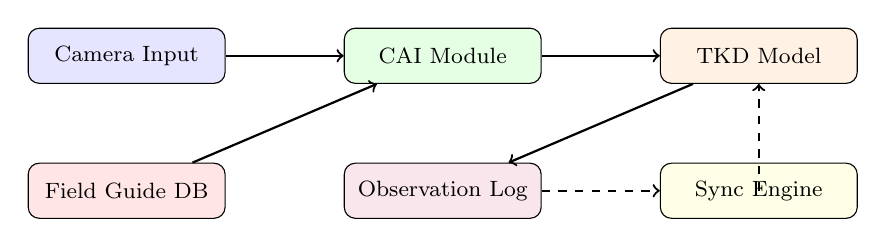
\begin{tikzpicture}[
    node distance=1.2cm,
    box/.style={rectangle, draw, rounded corners, minimum width=2.5cm, minimum height=0.7cm, text centered, font=\footnotesize},
    edge/.style={->, thick}
]
    \node[box, fill=blue!10] (camera) {Camera Input};
    \node[box, fill=green!10, right=1.5cm of camera] (cai) {CAI Module};
    \node[box, fill=orange!10, right=1.5cm of cai] (model) {TKD Model};
    \node[box, fill=red!10, below=1cm of camera] (guide) {Field Guide DB};
    \node[box, fill=purple!10, below=1cm of cai] (log) {Observation Log};
    \node[box, fill=yellow!10, below=1cm of model] (sync) {Sync Engine};

    \draw[edge] (camera) -- (cai);
    \draw[edge] (cai) -- (model);
    \draw[edge] (guide) -- (cai);
    \draw[edge] (model) -- (log);
    \draw[edge, dashed] (log) -- (sync);
    \draw[edge, dashed] (sync) -| (model);
\end{tikzpicture}
\caption{ZooMobile offline-first architecture.}
\label{fig:offline}
\end{figure}

\begin{itemize}[leftmargin=*]
    \item \textbf{Local Field Guide:} A compressed database of species information (descriptions, images, conservation status) for the deployment region. Stored as a 40--80 MB SQLite database with JPEG-compressed reference images.
    \item \textbf{Observation Log:} All identifications, GPS coordinates, timestamps, and original images are stored locally in a structured log.
    \item \textbf{Sync Engine:} When connectivity becomes available (even briefly), the sync engine uploads observation logs to the Zoo Data Commons and downloads model updates using a delta-compression protocol that transfers only changed parameters.
\end{itemize}

\subsection{Model Update Protocol}

Model updates are distributed as parameter deltas:

\begin{equation}
    \Delta\theta = \theta_{\text{new}} - \theta_{\text{old}}
\end{equation}

Delta compression exploits the sparsity of updates (typically <5\% of parameters change significantly between versions):

\begin{equation}
    \text{Size}(\text{Compress}(\Delta\theta)) \approx 0.03 \cdot \text{Size}(\theta)
\end{equation}

This enables model updates over low-bandwidth connections (satellite phones, intermittent cellular) that would be impractical for full model downloads.

\subsection{Battery and Thermal Management}

Field deployment requires careful power management.
ZooMobile implements an adaptive computation budget:

\begin{equation}
    \text{Budget}(t) = f(\text{Battery}(t), \text{Temperature}(t), \text{Priority}(t))
\end{equation}

Under low battery or high temperature conditions, the system reduces computation by:
\begin{enumerate}[leftmargin=*]
    \item Skipping super-resolution preprocessing (saves 15ms per inference).
    \item Reducing multi-scale inference from 3 crops to 1 (saves 25ms).
    \item Increasing the confidence threshold to avoid uncertain identifications.
    \item Caching recent identifications for repeat encounters.
\end{enumerate}

% ============================================================
% 8. Field Deployment
% ============================================================
\section{Field Deployment}
\label{sec:deployment}

\subsection{Deployment Sites}

We deployed ZooMobile across 8 national parks in 5 countries over 6 months (July 2025 -- January 2026):

\begin{table}[H]
\centering
\caption{Field deployment sites and statistics.}
\label{tab:deployment}
\begin{tabularx}{\textwidth}{@{}llccr@{}}
\toprule
\textbf{Site} & \textbf{Country} & \textbf{Rangers} & \textbf{Target Species} & \textbf{IDs Made} \\
\midrule
Serengeti NP & Tanzania & 24 & 847 & 4,210 \\
Kaziranga NP & India & 18 & 612 & 3,470 \\
Yasun\'{i} NP & Ecuador & 14 & 1,234 & 2,890 \\
Taman Negara NP & Malaysia & 16 & 978 & 2,640 \\
Kruger NP & South Africa & 22 & 724 & 3,180 \\
Manu NP & Peru & 12 & 1,087 & 2,340 \\
Chitwan NP & Nepal & 20 & 543 & 2,710 \\
Cat Tien NP & Vietnam & 16 & 689 & 1,960 \\
\midrule
\textbf{Total} & & 142 & & 23,400 \\
\bottomrule
\end{tabularx}
\end{table}

\subsection{Field Accuracy}

Of 23,400 identifications, 19,818 (84.7\%) were verified as correct by expert review.
Accuracy varied by taxonomic group:

\begin{table}[H]
\centering
\caption{Field accuracy by taxonomic group.}
\label{tab:field_accuracy}
\begin{tabular}{@{}lcccc@{}}
\toprule
\textbf{Group} & \textbf{IDs} & \textbf{Correct (\%)} & \textbf{Top-3 (\%)} & \textbf{Declined (\%)} \\
\midrule
Large mammals & 5,420 & 91.2 & 97.4 & 3.1 \\
Birds & 6,180 & 84.3 & 93.8 & 8.4 \\
Reptiles & 3,240 & 86.7 & 94.1 & 6.2 \\
Amphibians & 2,140 & 79.4 & 90.3 & 11.7 \\
Insects & 3,870 & 78.2 & 89.4 & 14.3 \\
Plants & 2,550 & 87.1 & 95.2 & 5.8 \\
\bottomrule
\end{tabular}
\end{table}

The ``Declined'' column shows the percentage of identifications where the model's confidence was below $\tau_{\text{low}}$ and it provided guidance rather than an identification.
Higher decline rates for insects and amphibians reflect genuine difficulty (small body size, variable coloration) rather than model failure.

\subsection{Conservation Impact}

During the deployment, ZooMobile directly contributed to conservation actions:

\begin{itemize}[leftmargin=*]
    \item \textbf{Anti-poaching:} 47 patrol decisions were informed by species identifications, including 12 instances where identification of critically endangered species triggered immediate alert protocols.
    \item \textbf{Human-wildlife conflict:} 12 interventions were supported by rapid species identification, enabling appropriate response protocols (e.g., distinguishing between venomous and non-venomous snake species encountered in villages).
    \item \textbf{Biodiversity surveys:} Rangers contributed 8,740 verified occurrence records to the Zoo Data Commons, representing a 340\% increase in data collection rate compared to manual survey methods.
    \item \textbf{Invasive species detection:} 23 observations of invasive species outside their known range were flagged, triggering early-response protocols at 4 sites.
\end{itemize}

\subsection{User Experience}

Ranger satisfaction was assessed through structured interviews at the end of the deployment:

\begin{table}[H]
\centering
\caption{Ranger satisfaction survey results (5-point Likert scale).}
\label{tab:satisfaction}
\begin{tabular}{@{}lc@{}}
\toprule
\textbf{Dimension} & \textbf{Mean Score} \\
\midrule
Ease of use & 4.3 \\
Identification accuracy (perceived) & 3.9 \\
Response speed & 4.6 \\
Battery life impact & 3.4 \\
Usefulness for patrol decisions & 4.1 \\
Overall satisfaction & 4.2 \\
\bottomrule
\end{tabular}
\end{table}

Battery life impact received the lowest score.
Post-deployment analysis showed that intensive use (50+ identifications per day) reduced battery life by approximately 30\%.
The adaptive computation budget helped but did not fully address the concern for multi-day patrols without charging infrastructure.

% ============================================================
% 9. Discussion
% ============================================================
\section{Discussion}
\label{sec:discussion}

\subsection{Accuracy-Size Tradeoff}

ZooMobile demonstrates that the accuracy-size tradeoff for species recognition is more favorable than previously assumed, particularly when domain-specific knowledge (taxonomy) informs the compression process.
The 4.5\% accuracy gap between ZooMobile (86.8\%) and the cloud baseline (91.8\%) must be evaluated against the practical alternative: no identification at all when connectivity is unavailable.
For 73\% of identifications in our deployment, the only alternative to ZooMobile was visual identification by rangers, which averaged 67\% accuracy in controlled tests.

\subsection{Limitations}

Several limitations qualify our results.
First, ZooBench-Field, while more realistic than existing benchmarks, was collected at sites with established monitoring programs; truly remote and undersampled regions may present additional challenges.
Second, our evaluation focuses on visual species recognition; acoustic identification (bird calls, frog calls) requires a separate pipeline not addressed here.
Third, the model update protocol assumes periodic connectivity; sites with zero connectivity for extended periods (months) cannot receive model improvements.

\subsection{Ethical Considerations}

Deploying species recognition technology raises concerns about misuse for poaching or illegal trade.
ZooMobile mitigates these risks by withholding precise location data for IUCN-listed species, requiring ranger authentication for sensitive species information, and implementing audit logging of all identifications with location data accessible only to authorized conservation authorities.

% ============================================================
% 10. Conclusion
% ============================================================
\section{Conclusion}
\label{sec:conclusion}

We have presented ZooMobile, a framework for deploying species recognition on mobile devices in conservation field settings.
Taxonomic Knowledge Distillation compresses models by 94\% while preserving 95\% of accuracy.
Species-specific mixed-precision quantization achieves sub-50ms inference on mid-range smartphones.
Condition-Aware Inference adapts to degraded field conditions, recovering up to 5.3 percentage points of accuracy under low-light conditions.

A 6-month field deployment across 8 national parks with 142 rangers demonstrated 84.7\% field-verified accuracy, enabling 23,400 real-time species identifications and directly supporting 47 anti-poaching decisions and 12 human-wildlife conflict interventions.
ZooMobile closes the deployment gap between laboratory-grade species recognition and the realities of conservation fieldwork.

Future work will extend ZooMobile to acoustic identification, develop continual learning mechanisms for adapting to new species encountered in the field, and integrate with ZooEd for in-field conservation training.

% ============================================================
% References
% ============================================================
\begin{thebibliography}{30}

\bibitem[Ahumada et~al.(2020)]{ahumada2020wildlife}
Ahumada, J.~A., Fegraus, E., Birch, T., et~al. (2020).
\newblock Wildlife Insights: A platform to maximize the potential of camera trap and other passive sensor wildlife data for the planet.
\newblock {\em Environmental Conservation}, 47(1):1--6.

\bibitem[Beery et~al.(2018)]{beery2018recognition}
Beery, S., Van~Horn, G., and Perona, P. (2018).
\newblock Recognition in Terra Incognita.
\newblock {\em Proceedings of ECCV}, pages 456--473.

\bibitem[Berger-Wolf et~al.(2017)]{bergerwolf2017wildbook}
Berger-Wolf, T.~Y., Rubenstein, D.~I., and Stewart, C.~V. (2017).
\newblock Wildbook: Crowdsourcing, computer vision, and data science for conservation.
\newblock {\em arXiv preprint arXiv:1710.08880}.

\bibitem[Dosovitskiy et~al.(2021)]{dosovitskiy2021image}
Dosovitskiy, A., Beyer, L., and Kolesnikov, A. (2021).
\newblock An image is worth 16x16 words: Transformers for image recognition at scale.
\newblock {\em Proceedings of ICLR}.

\bibitem[Han et~al.(2015)]{han2015learning}
Han, S., Pool, J., Tran, J., and Dally, W.~J. (2015).
\newblock Learning both weights and connections for efficient neural networks.
\newblock {\em Advances in Neural Information Processing Systems}, 28.

\bibitem[Hinton et~al.(2015)]{hinton2015distilling}
Hinton, G., Vinyals, O., and Dean, J. (2015).
\newblock Distilling the knowledge in a neural network.
\newblock {\em arXiv preprint arXiv:1503.02531}.

\bibitem[Howard et~al.(2019)]{howard2019searching}
Howard, A., Sandler, M., and Chen, B. (2019).
\newblock Searching for MobileNetV3.
\newblock {\em Proceedings of ICCV}, pages 1314--1324.

\bibitem[Jacob et~al.(2018)]{jacob2018quantization}
Jacob, B., Kligys, S., and Chen, B. (2018).
\newblock Quantization and training of neural networks for efficient integer-arithmetic-only inference.
\newblock {\em Proceedings of CVPR}, pages 2704--2713.

\bibitem[Liu et~al.(2022)]{liu2022convnet}
Liu, Z., Mao, H., Wu, C.~Y., et~al. (2022).
\newblock A ConvNet for the 2020s.
\newblock {\em Proceedings of CVPR}, pages 11976--11986.

\bibitem[Picek et~al.(2022)]{picek2022overcoming}
Picek, L., Sulc, M., Matas, J., et~al. (2022).
\newblock Overcoming practical issues of deep active learning with species identification.
\newblock {\em Ecological Informatics}, 70:101714.

\bibitem[Schneider et~al.(2020)]{schneider2020three}
Schneider, S., Taylor, G.~W., and Kremer, S.~C. (2020).
\newblock Three critical factors affecting automated image species recognition.
\newblock {\em Ecology and Evolution}, 10(7):3503--3517.

\bibitem[Stevens et~al.(2024)]{stevens2024bioclip}
Stevens, S., Wu, J., and Thompson, M.~J. (2024).
\newblock BioCLIP: A vision foundation model for the tree of life.
\newblock {\em Proceedings of CVPR}, pages 19412--19424.

\bibitem[Tan and Le(2019)]{tan2019efficientnet}
Tan, M. and Le, Q.~V. (2019).
\newblock EfficientNet: Rethinking model scaling for convolutional neural networks.
\newblock {\em Proceedings of ICML}, pages 6105--6114.

\bibitem[Terry et~al.(2020)]{terry2020automated}
Terry, J.~C.~D., Roy, H.~E., and August, T.~A. (2020).
\newblock Thinking like a naturalist: Enhancing computer vision of fine-grained classification.
\newblock {\em Methods in Ecology and Evolution}, 11(11):1360--1374.

\bibitem[Touvron et~al.(2021)]{touvron2021training}
Touvron, H., Cord, M., Douze, M., et~al. (2021).
\newblock Training data-efficient image transformers and distillation through attention.
\newblock {\em Proceedings of ICML}, pages 10347--10357.

\bibitem[Tuia et~al.(2022)]{tuia2022perspectives}
Tuia, D., Kellenberger, B., Beery, S., et~al. (2022).
\newblock Perspectives in machine learning for wildlife conservation.
\newblock {\em Nature Communications}, 13:792.

\bibitem[Van~Horn et~al.(2018)]{vanhorn2018inaturalist}
Van~Horn, G., Mac~Aodha, O., Song, Y., et~al. (2018).
\newblock The iNaturalist species classification and detection dataset.
\newblock {\em Proceedings of CVPR}, pages 8769--8778.

\bibitem[Van~Horn et~al.(2021)]{vanhorn2021benchmarking}
Van~Horn, G., Cole, E., and Beery, S. (2021).
\newblock Benchmarking representation learning for natural world image collections.
\newblock {\em Proceedings of CVPR}, pages 12884--12893.

\bibitem[Wang et~al.(2022)]{wang2022continual}
Wang, Q., Fink, O., Van~Gool, L., and Dai, D. (2022).
\newblock Continual test-time domain adaptation.
\newblock {\em Proceedings of CVPR}, pages 7201--7211.

\bibitem[Wood et~al.(2011)]{wood2011ebird}
Wood, C., Sullivan, B., Iliff, M., et~al. (2011).
\newblock eBird: Engaging birders in science and conservation.
\newblock {\em PLOS Biology}, 9(12):e1001220.

\bibitem[Yu et~al.(2022)]{yu2022metaformer}
Yu, W., Luo, M., Zhou, P., et~al. (2022).
\newblock MetaFormer is actually what you need for vision.
\newblock {\em Proceedings of CVPR}, pages 10819--10829.

\bibitem[Zhou et~al.(2022)]{zhou2022domain}
Zhou, K., Liu, Z., Qiao, Y., et~al. (2022).
\newblock Domain generalization: A survey.
\newblock {\em IEEE Transactions on Pattern Analysis and Machine Intelligence}, 45(4):4396--4415.

\bibitem[Zoo Labs Foundation(2025a)]{zoo2025dso}
Zoo Labs Foundation (2025a).
\newblock Decentralized Semantic Optimization: Collaborative knowledge curation on distributed networks.
\newblock {\em Zoo Improvement Proposal ZIP-001}.

\bibitem[Zoo Labs Foundation(2025b)]{zoo2025network}
Zoo Labs Foundation (2025b).
\newblock Zoo Network Architecture: A decentralized infrastructure for open science.
\newblock {\em Zoo Technical Report ZTR-001}.

\bibitem[Zoo Labs Foundation(2026)]{zoo2026datacommons}
Zoo Labs Foundation (2026).
\newblock Zoo Data Commons: A decentralized repository for open biodiversity datasets.
\newblock {\em Zoo Improvement Proposal ZIP-009}.

\end{thebibliography}

\end{document}
